\documentclass[aspectratio=169]{beamer}
\usetheme{metropolis}

\usepackage[utf8]{inputenc}
\usepackage[english]{babel}
\usepackage{booktabs}
\usepackage{listings}
\usepackage{color}

\usepackage{tikz}
\usetikzlibrary{shapes.geometric, arrows.meta, positioning, calc}

% Configuración para bloques de código
\definecolor{codegreen}{rgb}{0,0.6,0}
\definecolor{codegray}{rgb}{0.5,0.5,0.5}
\definecolor{codepurple}{rgb}{0.58,0,0.82}
\definecolor{backcolour}{rgb}{0.95,0.95,0.92}

\lstset{
	backgroundcolor=\color{backcolour},   
	commentstyle=\color{codegreen},
	keywordstyle=\color{magenta},
	numberstyle=\tiny\color{codegray},
	stringstyle=\color{codepurple},
	basicstyle=\ttfamily\footnotesize,
	breaklines=true,
	captionpos=b,                    
	keepspaces=true,                 
	showspaces=false,                
	showstringspaces=false,
	showtabs=false,                  
	tabsize=2
}

\title{LLMs \& VLMs course}
\subtitle{Preprocessing}
\author{Juan Irving Vasquez}
\date{\today}
\institute{Instituto Politécnico Nacional (IPN)}
\titlegraphic{
\includegraphics[height=1.2cm]{ipn-cidetec.png}\hspace{0.1cm}
\includegraphics[height=1.2cm]{escudoESCOM}}

\begin{document}
	
	\maketitle
	
	% --- Slide 1: Overview ---
\begin{frame}{The LLM Preprocessing}
	\begin{itemize}
		\item \textbf{Input:} Raw text (books, websites, code).
		\item \textbf{Goal:} Convert discrete linguistic symbols into numerical tensors suitable for deep learning.
		\item \textbf{Vectorization:}
		\begin{enumerate}
			\item Text normalization and cleaning.
			\item Tokenization: Breaking text into smaller units.
			\item Mapping: Converting tokens to integer IDs.
			
		\end{enumerate}
	\item \textbf{Embedding:} 
	\begin{itemize}
		\item Projecting IDs into a continuous vector space.
	\end{itemize}
	\end{itemize}
\end{frame}
	
	
% --- SLIDE 1 ---
\begin{frame}{Vectorization}
	\begin{columns}[T]
		% Left Column: Text and Example
		\begin{column}{0.45\textwidth}
			\begin{itemize}
				\item Deep learning models, being differentiable functions, can only process numeric tensors
				\item They can't take raw text as input.
				\item Vectorizing text is the process of transforming text into numeric tensors.
			\end{itemize}
			
			\vspace{0.3cm}
		\end{column}
		
		% Right Column: Image Space
		\begin{column}{0.55\textwidth}
			\centering
			\begin{figure}[h]
				\scriptsize
				\centering
				\begin{tikzpicture}[
					% Definición de estilos
					node distance=0.7cm,
					box/.style={
						rectangle, 
						draw=black, 
						fill=gray!15, 
						minimum width=3cm, 
						minimum height=0.5cm, 
						align=center,
						font=\sffamily
					},
					label_text/.style={
						font=\sffamily\bfseries,
						anchor=east,
						xshift=-0.5cm
					},
					arrow_label/.style={
						font=\sffamily\scriptsize,
						anchor=west,
						xshift=0.1cm
					},
					arrow/.style={
						-{Stealth[scale=1.2]},
						thick
					}
					]
					
					% Nodos (Cajas)
					\node [box] (text) {The cat sat on the mat.};
					\node [box, below=of text] (standardized) {the cat sat on the mat};
					\node [box, below=of standardized] (tokens) {"the", "cat", "sat", "on", "the", "mat"};
					\node [box, below=of tokens] (indices) {3, 26, 65, 9, 3, 133};
					
					% Nodo especial para los vectores (One-hot encoding)
					\node [box, below=of indices, minimum height=0.3cm, yshift=-0.2cm] (vectors) {
						\begin{tikzpicture}[scale=0.2]
							\foreach \x/\vals in {0/{0,0,0,1,0,0}, 1/{0,0,0,0,1,0}, 2/{0,1,0,0,0,0}, 3/{1,0,0,0,0,0}, 4/{0,0,0,0,1,0}, 5/{1,0,0,0,0,1}} {
								\draw[draw=black] (\x*1.2, 1.5) rectangle ++(0.8, 5);
								\foreach \y [count=\i] in \vals {
									\node at (\x*1.2 + 0.4, 7.4 - \i*0.7) {\tiny \y};
								}
							}
						\end{tikzpicture}
					};
					
					% Etiquetas a la izquierda [cite: 2, 6, 10, 14, 18]
					\node [label_text] at (text.west) {Text};
					\node [label_text] at (standardized.west) {Standardized text};
					\node [label_text] at (tokens.west) {Tokens};
					\node [label_text] at (indices.west) {Token indices};
					\node [label_text, align=right] at (vectors.west) {Vector\\encoding\\of indices};
					
					% Flechas y etiquetas a la derecha [cite: 5, 8, 13, 17]
					\draw [arrow] (text) -- (standardized) node[midway, arrow_label] {Standardization};
					\draw [arrow] (standardized) -- (tokens) node[midway, arrow_label] {Tokenization};
					\draw [arrow] (tokens) -- (indices) node[midway, arrow_label] {Indexing};
					\draw [arrow] (indices) -- (vectors) node[midway, arrow_label] {One-hot encoding};
					
				\end{tikzpicture}
				\caption{Data vectorization.}
			\end{figure}
		\end{column}
	\end{columns}
\end{frame}


%% --- SLIDE 3 & 4 ---
%\begin{frame}{Text Processing Models}
%	There are two kinds of text-processing models:
%	\begin{itemize}
%		\item \textbf{Sequence models:} care about word order (uses word-level tokenization).
%		\item \textbf{Bag-of-words models:} treat input words as a set, discarding their original order (uses N-gram tokenization).
%	\end{itemize}
%	
%	\begin{exampleblock}{N-grams Example}
%		"the cat sat on the mat." $\rightarrow$ \{"the", "the cat", "cat", "cat sat", "sat", "sat on", ...\}
%	\end{exampleblock}
%\end{frame}


	% --- SLIDE 2 ---
\begin{frame}{Tokenization}
	There are different levels for decomposing text:
	\begin{itemize}
		\item \textbf{Word-level tokenization:} tokens are space-separated (or punctuation-separated) substrings.
		\item \textbf{N-gram tokenization:} tokens are groups of N consecutive words (e.g., "the cat" is a 2-gram or bigram).
		\item \textbf{Character-level tokenization:} each character is its own token.
		\item \textbf{Subword-level (Standard for LLMs):}
		\begin{itemize}
			\item Examples: \textbf{Byte Pair Encoding (BPE)}, WordPiece.
			\item Breaks rare words into sub-parts (e.g., "unhappy" $\rightarrow$ "un", "happy").
			\item Balance between vocabulary size and sequence length.
		\end{itemize}
	\end{itemize}
\end{frame}


% --- Slide 3: Byte Pair Encoding (BPE) ---
\begin{frame}{Byte Pair Encoding (BPE) Mechanism}
	BPE is the algorithm used by GPT-2, GPT-3, and Llama.
	\begin{enumerate}
		\item Start with individual characters as the initial vocabulary.
		\item Iteratively merge the most frequently occurring adjacent pair of tokens into a new single token.
		\item Repeat until a target vocabulary size is reached.
	\end{enumerate}
	\textbf{Advantages:}
	\begin{itemize}
		\item Efficiently handles unknown words by falling back to character-level components.
		\item Reduces the total number of tokens per sequence compared to character-level.
	\end{itemize}
\end{frame}


\begin{frame}{Byte Pair Encoding (BPE) Mechanism}
% TODO: \usepackage{graphicx} required
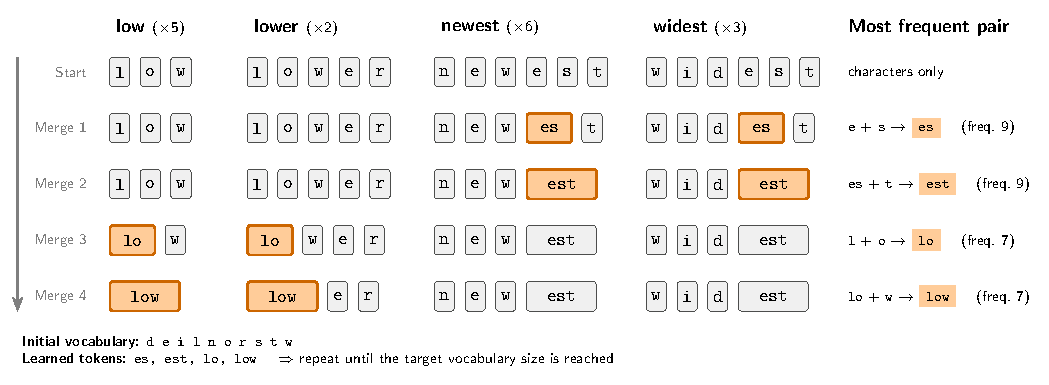
\includegraphics[height=0.65\textheight]{figures/bpe}
\end{frame}


% --- Slide 4: Special Tokens ---
\begin{frame}{Special Tokens and size}
	To help the model understand structure, we introduce non-text tokens:
	\begin{itemize}
		\item \texttt{<|endoftext|>}: Marks the end of a document or sequence (crucial for GPT-style models).
		\item \texttt{<|unk|>}: Represents words not in the vocabulary.
		\item \texttt{<|pad|>}: Used to ensure sequences in a batch have the same length.
	\end{itemize}

	Then the vocabulary is:
	\begin{equation}
		V = \{ \texttt{t}_i \}
	\end{equation}
	where $\texttt{t}_i$ is a token such as "low"
	\begin{equation}
		vocabulary\_size = |V|
	\end{equation}
	GPT-2 small: $|V| = 50{,}257$
%	\textbf{Context Window:} The maximum number of tokens an LLM can process at once (e.g., 2048, 4096, or 128k).
\end{frame}


% --- SLIDE 5 ---
\begin{frame}[fragile]{Vocabulary Indexing}
	\begin{itemize}
		\item Once text is split into tokens, you need to encode each into a numerical and vector representation.
		\begin{equation}
			O = \texttt{OneHot}(ID(\texttt{t}))
		\end{equation}
		where
		\begin{equation}
			\texttt{OneHot}:\mathbb{Z} \rightarrow \mathbb{B}^{|V|}
		\end{equation}
		\item In practice, you build an index of all terms in the training data (the "vocabulary") and assign a unique integer to each entry.
	\end{itemize}

\begin{figure}
	\centering
	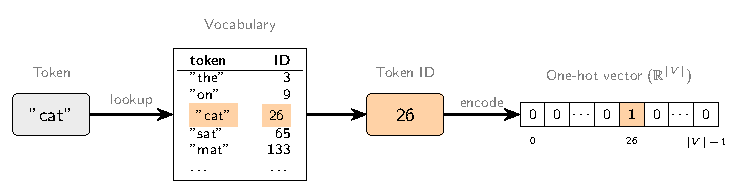
\includegraphics[height=0.4\textheight]{figures/indexing}
\end{figure}
\end{frame}
	

	
% --- Slide 2: Tokenization Strategies ---
%	\begin{frame}{Tokenization Strategies}
%		How should we represent language units?
%		\begin{itemize}
%			\item \textbf{Word-level:} Large vocabulary, struggles with Out-Of-Vocabulary (OOV) words and morphology.
%			\item \textbf{Character-level:} Tiny vocabulary, but sequences become extremely long (losing semantic density).			
%		\end{itemize}
%	\end{frame}


	

% --- Slide: Text Embeddings ---
\begin{frame}{Text Embeddings}
	\begin{columns}
		\column{0.5\textwidth}

		\begin{itemize}
			\item Allow us to manipulate word representations in meaningful ways.
			\item We can find a word similar to another, or blend two words to find one in between.
		\end{itemize}
		
		\column{0.5\textwidth}
		\centering
		% Placeholder for embedding space image
		\centering
		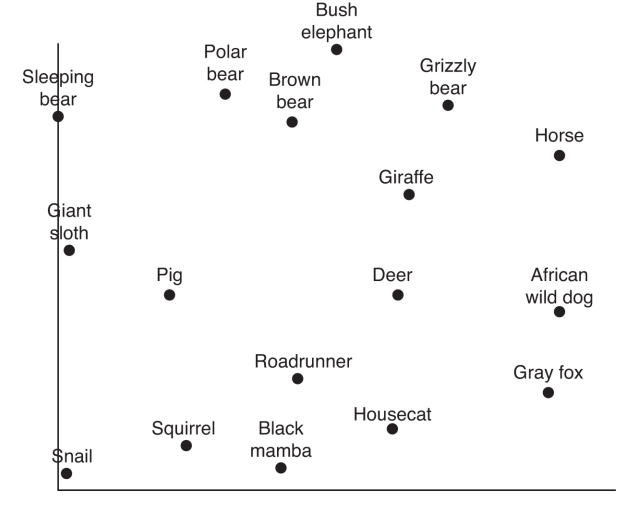
\includegraphics[width=\textwidth]{figures/embedspace.png}
	\end{columns}
\end{frame}



% --- Slide: Embeddings arithmetic ---
\begin{frame}{Embeddings Arithmetic}
	Embeddings allow for geometric vector operations:
	
	\centering
	
	\begin{figure}
		\centering
		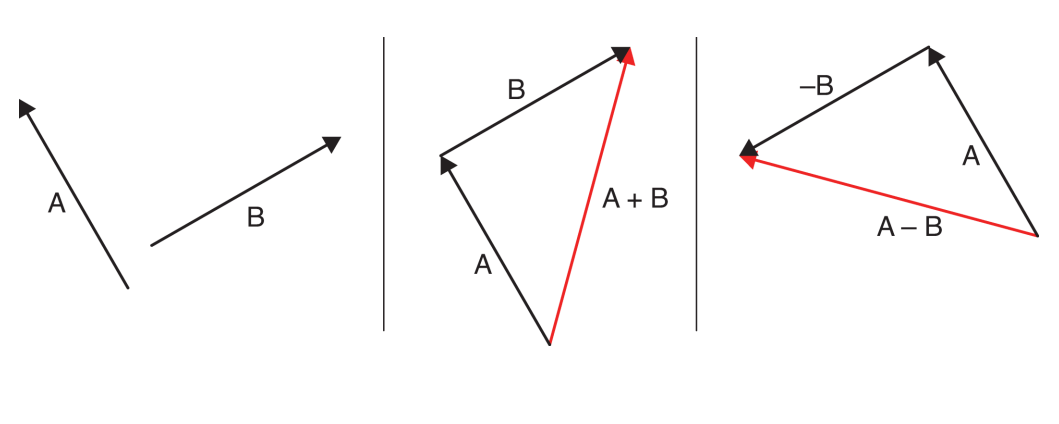
\includegraphics[width=0.7\linewidth]{figures/enbedarith}
		\caption{Embedding arithmetics}
		\label{fig:enbedarith}
	\end{figure}
	
	\small (Visually represented as vector addition and subtraction in space).
\end{frame}



% --- Slide: Linear Structure ---
\begin{frame}{Linear Structure of Embeddings}
	Surprisingly, many semantic and syntactic relationships are (almost) linear in the word vector space.
	
	\begin{block}{Semantic Relationships}
		$$v(king) - v(man) + v(woman) \approx v(queen)$$
		\tiny
	\end{block}
	
	\begin{block}{Syntactic Relationships}
		$$v(kings) - v(king) + v(queen) \approx v(queens)$$
		\tiny
	\end{block}
	
	\vfill
	\tiny Source: Mikolov, Tomas, et al. "Efficient estimation of word representations in vector space." arXiv (2013).
\end{frame}

% --- Slide: Embedding words ---
\begin{frame}{Word Embeddings}
	\begin{itemize}
		\item A word embedding represents a word as a vector of hundreds of dimensions.
		\begin{equation}
			\texttt{Embedding}(O):\mathbb{B}^{|V|} \rightarrow \mathbb{R}^{d_{model}}
		\end{equation}
		\begin{equation}
			\textbf{e} = \texttt{Embedding}(O)
		\end{equation}
	\item In Vaswani et al $d_{\text{model}} = 512$, in GPT2 $d_{\text{model}} = 768$
		\item Instead of assigning a single number, the algorithm assigns a list of numbers representing its coordinates in a huge space.
		\item The algorithm is called an \textit{embedder}, and the process is called \textit{embedding}.
		\item Instead of processing zero-dimensional tensors (single numbers), the system processes one-dimensional tensors (lists of numbers).
	\end{itemize}
\end{frame}


% --- Slide: Comparing embeddings ---
\begin{frame}{Comparing Embeddings by Similarity}
	\begin{columns}[c] % El argumento [c] alinea el contenido verticalmente en el centro
		
		% Primera Columna: Imagen
		\begin{column}{0.6\textwidth}
			\begin{figure}
				\centering
				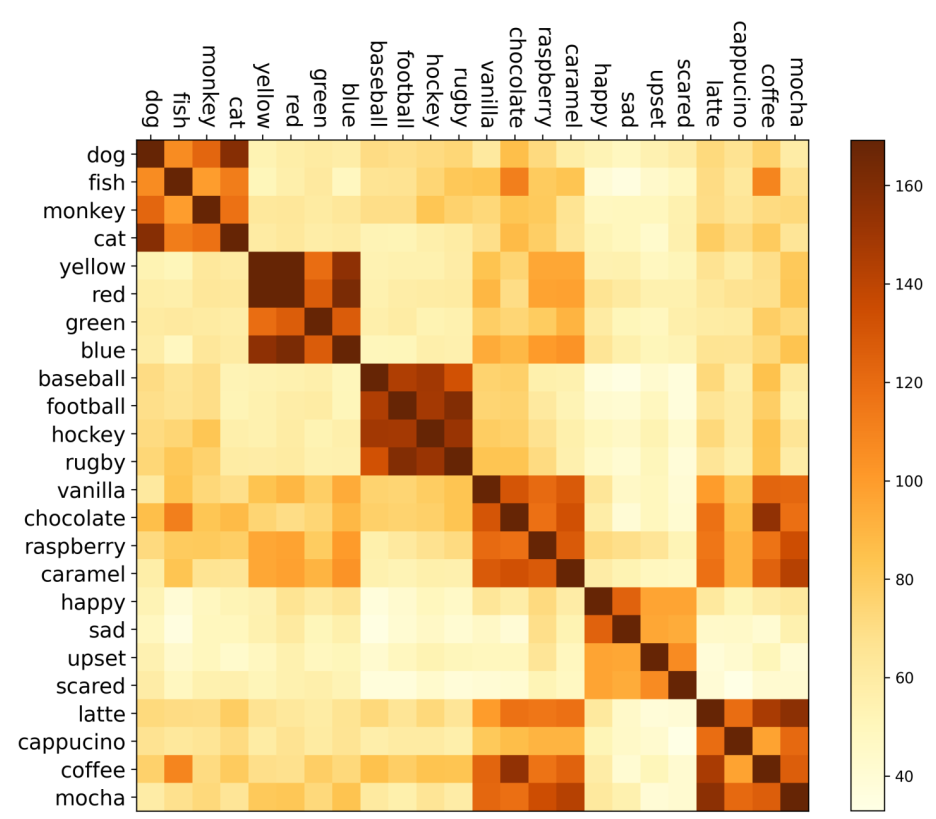
\includegraphics[width=0.8\linewidth]{figures/embed_compar} % Ajustado a \linewidth para que se adapte bien a su columna
				\caption{Word embedding correlation}
				\label{fig:embedcompar}
			\end{figure}
		\end{column}
		
		% Segunda Columna: Texto y Lista
		\begin{column}{0.4\textwidth}
			\textbf{Famous Algorithms:}
			\begin{itemize}
				\item GloVe (2013).
				\item Word2vec (2014).
				\item fastText (2020).
			\end{itemize}
		\end{column}
	\end{columns}
\end{frame}


% --- Slide: Embed sentences ---
\begin{frame}{Sentence Embeddings\footnote{Cer, Daniel, et al. "Universal Sentence Encoder." arXiv (2018).}}
	\begin{figure}
		\centering
		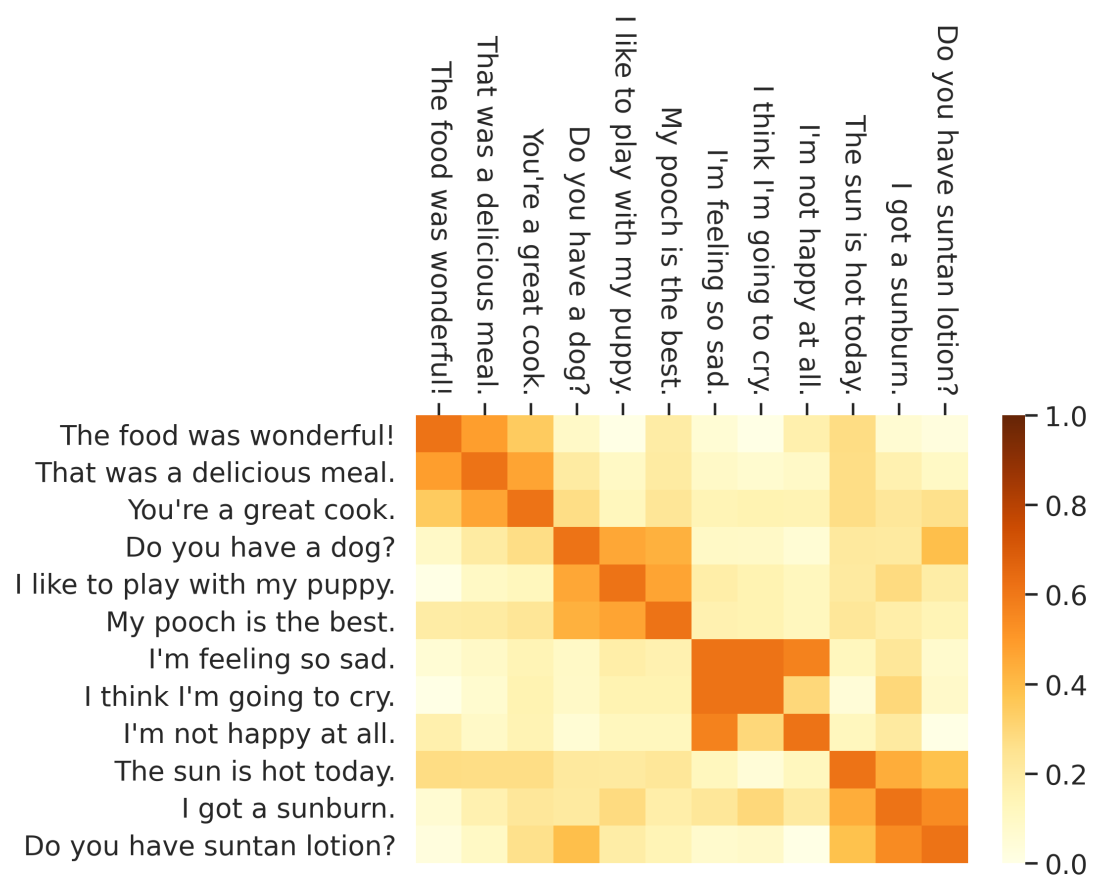
\includegraphics[width=0.5\linewidth]{figures/embedsent}
		\caption{Correlation of embedded sentences}
		\label{fig:embedsent}
	\end{figure}
\end{frame}


% --- Slide: Problem with Word embeddings ---
\begin{frame}{Dynamic Embeddings}
	Many languages have words with different meanings that are written the same way (homonyms).
	
	\textbf{The case of the word "train":}
	\begin{itemize}
		\item Noun: "I rode on a \textbf{train}".
		\item Verb: "I like to \textbf{train} dogs".
	\end{itemize}
	
	\begin{alertblock}{Limitation}
		If we assign a single static embedding to "train", we mix two entirely different ideas. We need to distinguish meanings based on context.
	\end{alertblock}
	
	\textit{This leads us to the need for contextualized embeddings (like ELMo and Transformers).}
\end{frame}
	
	
% --- Slide 6: Token Embeddings ---
%	\begin{frame}{Token Embeddings}
%		\begin{itemize}
%			\item \textbf{Identity Mapping:} Integer IDs carry no semantic meaning (ID 5 is not "closer" to ID 6).
%			\item \textbf{Embedding Layer:} A lookup table of size $(VocabSize \times EmbeddingDimension)$.
%			\item \textbf{Projection:} Each token ID is mapped to a vector in $\mathbb{R}^d$ (e.g., $d=768$ for GPT-2).
%			\item These vectors are \textbf{learnable parameters} updated during backpropagation.
%		\end{itemize}
%	\end{frame}


% --- GPT-2 embedding: forward pass ---
\begin{frame}{GPT-2 Embeddings: Forward Pass}
	\small
	
	\begin{block}{Learnable matrices}
		\[
		W_E \in \mathbb{R}^{|V| \times d_{\text{model}}} \quad (\texttt{wte})
		\] 
	\end{block}
	
	\textbf{Embedding of the token t at position $ID$} (row lookup):
	\begin{equation}
		\texttt{Embedding}_{GPT2}(O) = O^{\top} W_E 
	\end{equation}
	 $$W_E[ID(\texttt{t})]$$
	\textbf{Matrix form} for the whole sequence:
	\begin{equation}
		\underbrace{\mathbf{O}\,W_E}_{n \times d_{\text{model}}} 
		\qquad \mathbf{O} \in \{0,1\}^{n \times |V|} \text{ (one-hot rows)}
	\end{equation}
	where $n$ is the input lenght
\end{frame}


	
	
% --- Slide 7: Positional Embeddings ---
	\begin{frame}{Adding Order: Positional Ecoding}
		Since the Transformer architecture is permutation-invariant (it processes all tokens in parallel), it doesn't "know" the position of a token.
		\begin{block}{The Solution}
			Add (or concatenate) a position-dependent vector to the token embedding.
		\end{block}
	\begin{itemize}
			\item \textbf{Absolute Positional Encodings:} Fixed sine/cosine functions or learnable vectors for each index $[0, 1, ..., MaxContext]$.
			\item \textbf{Relative Positional Encodings:} Focus on the distance between tokens (used in more recent architectures like RoPE).
	\end{itemize}
\end{frame}


\begin{frame}
	\frametitle{Absolute positional encoding}
	\begin{equation}
		X = \texttt{Embedding}(\textbf{e}) + PE(d_{\text{model}})
	\end{equation}
\begin{center}
	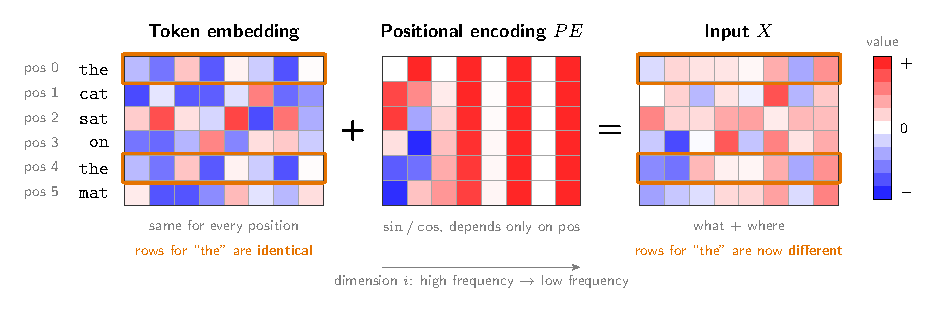
\includegraphics[height=0.6\textheight]{figures/pe_absolute}
\end{center}
\end{frame}



\begin{frame}
	\frametitle{Absolute positional encoding}
	\begin{equation*}
		X = Embedding(\textbf{Token}) + PE(d_{\text{model}})
	\end{equation*}
	
	\begin{columns}[c]
		% --- Columna izquierda: fórmulas ---
		\begin{column}{0.42\textwidth}
			\small
			For a given position $\text{pos}$ and a dimension index $i$ within the embedding vector:
			\begin{equation}
				PE_{(\text{pos}, 2i)} = \sin\left(\frac{\text{pos}}{10000^{\frac{2i}{d_{\text{model}}}}}\right)
			\end{equation}
			\begin{equation}
				PE_{(\text{pos}, 2i+1)} = \cos\left(\frac{\text{pos}}{10000^{\frac{2i}{d_{\text{model}}}}}\right)
			\end{equation}
		\end{column}
		
		% --- Columna derecha: figura ---
		\begin{column}{0.58\textwidth}
			\centering
			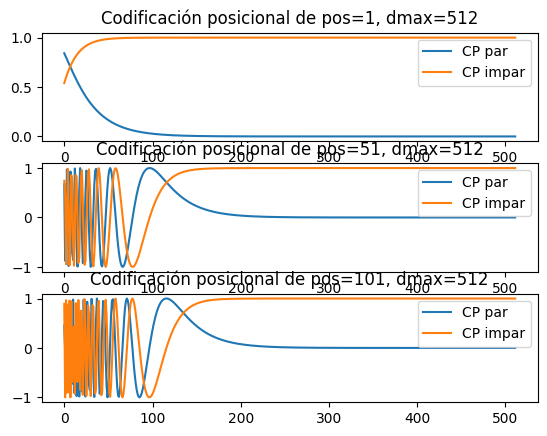
\includegraphics[width=0.7\linewidth]{figures/pe_example}
		\end{column}
	\end{columns}
\end{frame}



\begin{frame}{GPT-2 Positional encoding}
	
	\begin{block}{Learnable matrices}
		\[
		W_E \in \mathbb{R}^{|V| \times d_{\text{model}}} \quad (\texttt{wte}), \qquad
		W_P \in \mathbb{R}^{n_{\text{ctx}} \times d_{\text{model}}} \quad (\texttt{wpe})
		\]
	\end{block}
	
	\textbf{Embedding of the token at position $pos$}:
	\begin{equation}
		x_pos = W_E[pos] + W_P[pos] = O^{\top} W_E + O^{\top} W_P
	\end{equation}
	
	\textbf{Matrix form} for the whole sequence:
	\begin{equation}
		X = \underbrace{\mathbf{O}\,W_E}_{n \times d_{\text{model}}} + \underbrace{W_P[0\!:\!n]}_{n \times d_{\text{model}}},
		\qquad \mathbf{O} \in \{0,1\}^{n \times |V|} \text{ (one-hot rows)}
	\end{equation}
\end{frame}


\begin{frame}{GPT-2 Preprocessing}
\begin{center}
	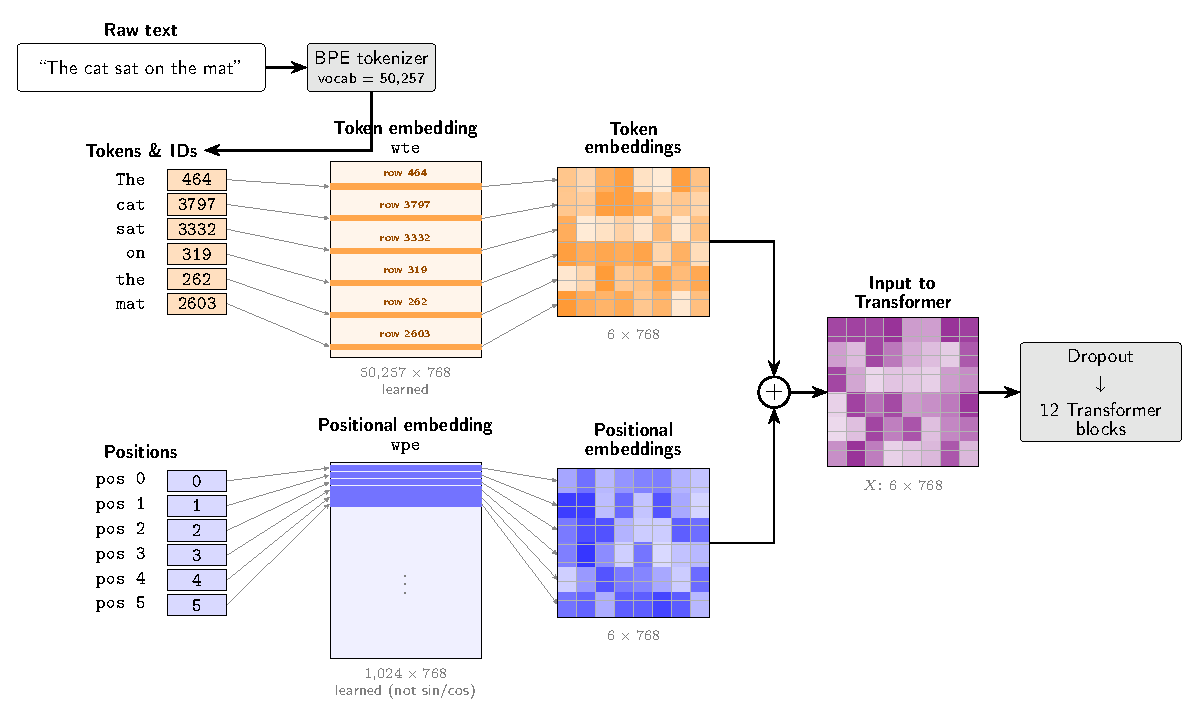
\includegraphics[height=0.95\textheight]{figures/gpt2_prep}
\end{center}
\end{frame}


% --- Slide 5: Data Sampling with Sliding Window ---
\begin{frame}[fragile]{Sliding Window for Training}
	LLMs are trained to predict the \textit{next} token. We use a sliding window to create input-target pairs.
	\vspace{0.3cm}
	\begin{lstlisting}[language=Python]
		# Input:  [1, 2, 3, 4, 5]
		# Window size = 4
		x = [1, 2, 3, 4] # Input sequence
		y = [2, 3, 4, 5] # Target sequence (shifted by 1)
	\end{lstlisting}
	\begin{itemize}
		\item For each position $i$ in the input, the model learns that the ground truth is the token at $i+1$.
	\end{itemize}
\end{frame}
	
	
%	% --- Slide 8: Data Loaders and Tensors ---
%	\begin{frame}{Input Tensors for PyTorch}
%		For a batch of text, the input tensor usually has the shape:
%		\[ [BatchSize, ContextLength, EmbeddingDimension] \]
%		\begin{itemize}
%			\item \textbf{Batching:} Processing multiple sequences in parallel to maximize GPU utilization.
%			\item \textbf{Padding:} If sequences have different lengths, they are padded to match the longest one in the batch.
%		\end{itemize}
%	\end{frame}
	
	\begin{frame}[standout]
		¿Questions?
	\end{frame}
	
\end{document}